\documentclass[aspectratio=169, 11pt]{beamer}

% --- Preamble & Fonts ---
% Removed fontspec commands as they often cause issues in limited compilation environments.
% The default beamer fonts should be sufficient for stability.
% If custom fonts are critical, we might need to resort to a different configuration.
\usepackage{amsmath}
\usepackage{algorithm}
\usepackage{algpseudocode}
\usepackage{tikz}

% --- TikZ & Beamer Overlay Setup ---
\tikzset{
  alt/.code args={<#1>#2#3}{%
    \alt<#1>{\pgfkeysalso{#2}}{\pgfkeysalso{#3}}%
  },
  bst/.style={
    circle, draw, fill=blue!10,
    minimum size=8mm, inner sep=0pt,
    font=\bfseries, line width=0.8pt
  },
  highlight/.style args={<#1>}{%
    alt=<#1>{
      opacity=1, text opacity=1,
      fill opacity=1, draw opacity=1,
      line width=1.5pt,
      color=blue!60!black, fill=blue!20
    }{
      opacity=0.3, text opacity=0.3,
      fill opacity=0.3, draw opacity=0.3
    }
  },
  level/.style={sibling distance=60mm/#1}
}

\title{Arbre de Recherche Binaire — Recherche}
\subtitle{Exemple de Recherche}
\author{Algorithmes et Pensée Computationnelle \newline \newline  {\small UNIL — École des Sciences Criminelles}}
\date{}

\begin{document}

\begin{frame}
\titlepage
\end{frame}


\begin{frame}
\begin{algorithm}[H]
\caption{TREE-SEARCH($x, k$)}
\begin{algorithmic}[1]
\If {$x == \text{NIL}$ or $k == x.key$}
    \State \textbf{return} $x$
\EndIf
\If {$k < x.key$}
    \State \textbf{return} $\text{TREE-SEARCH}(x.left, k)$
\Else
    \State \textbf{return} $\text{TREE-SEARCH}(x.right, k)$
\EndIf
\end{algorithmic}
\end{algorithm}

L'algorithme effectue une recherche récursive d'un nœud avec clé $k$ dans un arbre de recherche binaire depuis le nœud $x$.\newline 

Dans cet exemple, nous prenons $k$=11.

\end{frame}

% --- The Frame ---
\begin{frame}{Recherche de la valeur 11}
    \centering
    
    % We set the default opacity for the whole picture to 0.3.
    % The 'highlight' style will override this to 1.0 for active nodes.
    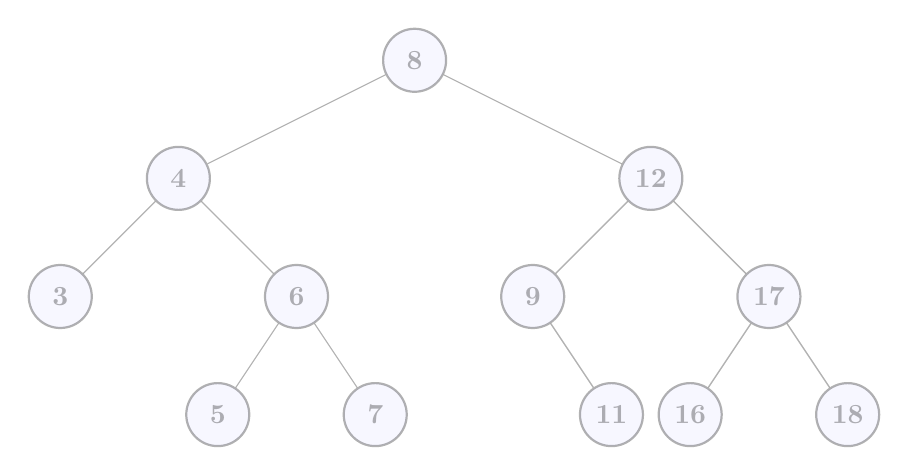
\begin{tikzpicture}[
  level distance=15mm,
  opacity=0.3, text opacity=0.3, fill opacity=0.3, draw opacity=0.3,
  every node/.style={bst},          % <-- FORCE bst on ALL nodes
  every child/.style={opacity=0.3, draw opacity=0.3}
]
    % --- ROOT NODE (8) ---
    % Active from Slide 1 onwards
    \node [bst, highlight=<1->] {8}
        % --- LEFT SUBTREE (4) ---
        % Not part of the path to 11, so no highlight style applied (remains dim)
        child { node [bst] {4}
            child { node [bst] {3} }
            child { node [bst] {6}
                child { node [bst] {5} }
                child { node [bst] {7} }
            }
        }
        % --- RIGHT SUBTREE (12) ---
        % 11 > 8, so we go right. Active from Slide 2 onwards.
        child { node [bst, highlight=<2->] {12}
            % 11 < 12, so we go left. Active from Slide 3 onwards.
            child { node [bst, draw=black, highlight=<3->] {9} 
                % Added draw opacity to child[missing] edge to ensure it remains invisible.
                child[missing, draw opacity=0] { node {} }
                % 11 > 9, so we go right. Found it! Active from Slide 4.
                child { node [bst, draw=black, highlight=<4->] {11} 
                    edge from parent [draw opacity=0.3, opacity=0.3, line width=0.5pt, color=black!60!black, highlight=<4->] % Highlight edge 9->11
                }
                edge from parent [draw opacity=0.3, opacity=0.3, line width=0.5pt, color=black!60!black, highlight=<3->] % Highlight edge 12->9
            } 
            child { node [bst, draw=black] {17}
                child { node [bst] {16} }
                child { node [bst, fill=blue!10] {18} }
                edge from parent [draw opacity=0.3, opacity=0.3, line width=0.5pt, color=black!60!black]
            }
            edge from parent [highlight=<2->] % Highlight edge 8->12
        };

    \end{tikzpicture}

    \vspace{1cm}
    
    % Dynamic text description at the bottom
    % \begin{itemize}
    %     \item<1-> \textbf{Start at Root (8)}: Target 11 is greater than 8. Go Right.
    %     \item<2-> \textbf{Visit 12}: Target 11 is less than 12. Go Left.
    %     \item<3-> \textbf{Visit 9}: Target 11 is greater than 9. Go Right.
    %     \item<4-> \textbf{Found 11}: Search successful.
    % \end{itemize}
\begin{itemize}
\item<1-> Ordre des visites: \only<1>{[8]}\only<2>{[8, 12]}\only<3>{[8, 12, 9]}\only<4>{[8, 12, 9, 11]}
\item<2-> \only<2>{11 $>$ 8  $\Rightarrow$ Sous-arbre de 8 à droite} \only<3>{11 $<$ 12  $\Rightarrow$ Sous-arbre de 12 à gauche} \only<4>{11 $>$ 9  $\Rightarrow$ Sous-arbre de 9 à droite}
\end{itemize}
\end{frame}

\end{document}